\documentclass{article}
\usepackage{listings, xcolor, graphicx, inconsolata, amsmath}
\setlength{\parindent}{0pt}

\definecolor{lgray}{rgb}{0.95, 0.95, 0.95}
\definecolor{lgray2}{rgb}{0.75, 0.75, 0.75}

\lstset{
  language=C++,
  aboveskip=10pt,
  belowskip=10pt,
  frame=leftline,
  xleftmargin=15pt,
  framexleftmargin=20pt,
  breaklines=true,
  basicstyle=\small,
  showstringspaces=false,
  backgroundcolor=\color{lgray},
  rulecolor=\color{lgray2},
  basicstyle=\ttfamily\footnotesize,
  keywordstyle=\color{blue},
  stringstyle=\color{red},
  commentstyle=\color{green},
  numbers=left,               
  numberstyle=\tiny\color{gray},
  stepnumber=1
}

\title{CS135; 1D Arrays and Strings}
\author{Gael Zarco}
\date{\today}

\begin{document}

\maketitle

\textbf{Structured Data Types} contain data where each item is a collection of
other data items.
\begin{itemize}
  \item Simple data structures are the building blocks of structured data types.
\end{itemize}

% SECTION 1 %
\section{Arrays}
An \textbf{Array} is a collection of a fixed number of components (also called
elements) all of the same data type and in contigous (adjacent) memory space. A
\textbf{One-Dimensional Array} is an array in which the components are arranged
in a list form.

\begin{lstlisting}[caption={1D Array Syntax}]
  dataType arrayName[intExp];

  // Example
  int list[5];    // Declared array 'list' of 10 elements
\end{lstlisting}

\texttt{intExp} specifies the number of components in the array and can be any
constant expression that evaluates to a positive integer. The Example above
delcares an array \texttt{list} of \textit{10} components.

\begin{itemize}
  \item The components are \texttt{list[0], list[1], ..., list[9]}.
  \item Declares a total of 10 variables
\end{itemize}

\begin{center}
    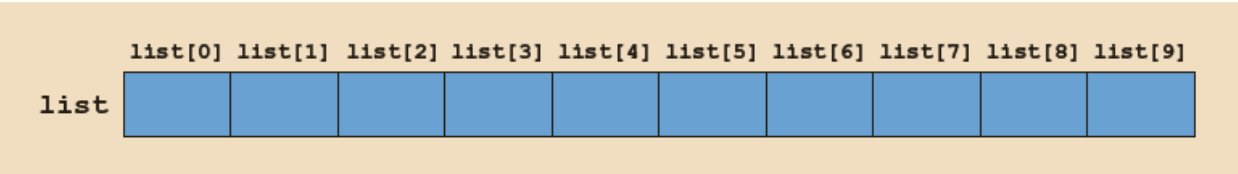
\includegraphics[width=0.9\textwidth]{1d-arr-vars.png}
\end{center}

\begin{lstlisting}[caption={1D Array Assignment}]
  list[5] = 34;
\end{lstlisting}

This expression stores \textit{34} in \texttt{list[5]}, which is the
\textit{sixth} component of the array \texttt{list}.

\begin{itemize}
  \item You can use \texttt{i} to index into an array.
  \begin {itemize}
    \item \texttt{list[i]}
  \end{itemize}
\end{itemize}

\begin{center}
    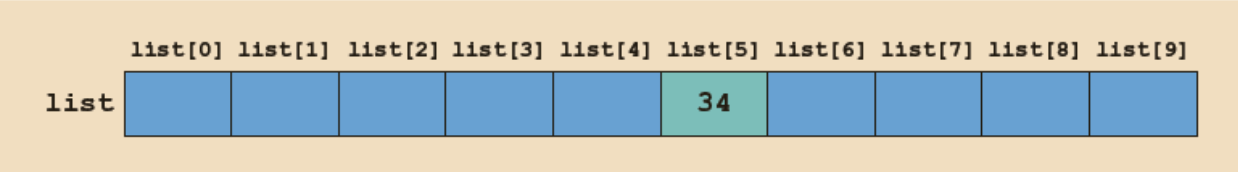
\includegraphics[width=0.9\textwidth]{1d-arr-var-assign.png}
\end{center}

\begin{lstlisting}[caption={1D Array Assignment Cont}]
  list[3] = 10;
  list[6] = 35;

  // Add the contents of list[3] and list[6] and store in list[5]
  list[5] = list[3] + list[6];
\end{lstlisting}

\begin{center}
    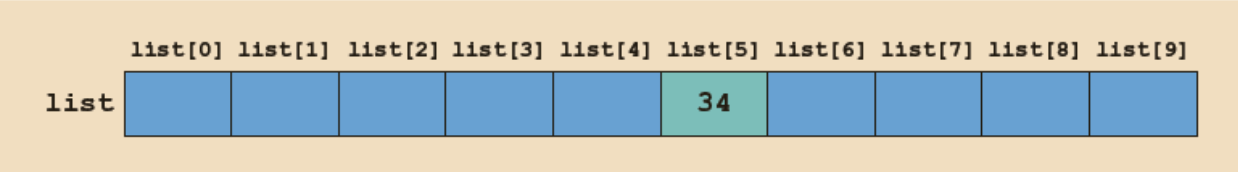
\includegraphics[width=0.9\textwidth]{1d-arr-var-assign.png}
\end{center}

% SECTION 1.1 %
\subsection{Processing One-Dimensional Arrays}

\begin{lstlisting}[caption={Read Data Into 1D Array}]
  for (i = 0; i < 10; i++)
    cin >> list[i];
\end{lstlisting}

\begin{lstlisting}[caption={Print Data From 1D Array}]
  for (i = 0; i < 10; i++)
    cout << list[i];
\end{lstlisting}

\begin{lstlisting}[caption={Find Sum \& Avg From 1D Array}]
  int sum = 0;
  int avg;

  for (i = 0; i < 10; i++)
    sum = sum + list[i]; 

  avg = sum / 10;
\end{lstlisting}

\begin{lstlisting}[caption={Find Largest Element in 1D Array}]
  int maxIdx = 0;

  for (int i = 1; i < 10; i++)
    if (list[maxIdx] < list[i])
      maxIdx = i;

  int largestInt = list[maxIdx];
\end{lstlisting}

% SECTION 1.2 %
\subsection{Array Index Out of Bounds}

\begin{lstlisting}[caption={Array Index Example}]
  double num[10];
  int i;
\end{lstlisting}

The component \texttt{num[i]} is \textit{valid} or \textbf{In Bounds} if
\texttt{index}:
\begin{itemize}
  \item $0 \leq \text{index} \leq \text{ARRAY\_SIZE} - 1$.
  \item \texttt{index} is not negative or greater than $\text{ARRAY\_SIZE} - 1$.
  \begin{itemize}
    \item It is \textbf{Out of Bounds} in this event.
    \item C++ does not check whether the index value is within range; this is
      the programmer's responsibility.
  \end{itemize}
\end{itemize}

% SECTION 1.3 %
\subsection{Array Initialization During Declaration}
An array can be initialized while being declared

\begin{lstlisting}[caption={Array Initialization Example}]
  double sales[5] = {12.25, 32.50, 16.90, 23, 45.68};

  // Not necessary to specify the size when initializing
  double sales[] = {12.25, 32.50, 16.90, 23, 45.68};
\end{lstlisting}

% SECTION 1.4 %
\subsection{Partial Initialization of Arrays During Declaration}

\begin{lstlisting}[caption={Partial Array Initialization}]
  int list[10] = {5, 6, 3};
\end{lstlisting}

The first three components of \texttt{list} are \texttt{list[0] = 5, list[1] =
6, list[2] = 3}, and the rest are set to the default of 0.

% SECTION 1.5 %
\subsection{Restrictions on Array Processing}
C++ does not allow \textbf{Aggregate Operations} on an array. Aggregate
operations on an array are any operations that manipulate the entire array as a single unit.

\begin{lstlisting}[caption={Illegal Aggregate Operation on Array}]
  int myList[5] = {0, 4, 8, 12, 16};
  int yourList[5];

  // illegal
  yourList = myList;
\end{lstlisting}

% SECTION 1.6 %
\subsection{Arrays as Parameters to Functions}
In C++, arrays are passed as parameters to functions by \textbf{Reference Only}.
You do \textbf{not} use the \texttt{\&} symbol when declaring an array as a
formal parameter.

\begin{lstlisting}[caption={Arrays as Formal Parameters}]
  void initialize(int list[], int listSize);
\end{lstlisting}

% SECTION 1.7 %
\subsection{Constant Arrays as Formal Parameters}
You can use \texttt{const} keyword in the declaration of a formal param to
prevent the function from changing the actual param.

\begin{lstlisting}[caption={Constant Arrays as Formal Parameters}]
  void foo(int x[], const int y[], int sizeX, int sizeY);
\end{lstlisting}

% SECTION 1.8 %
\subsection{Base Address of an Array and Array in Computer Memory}
The \textbf{Base Address} of an array is the address (memory location) of the
first array component.
\begin{itemize}
  \item In 1D arrays, the base address is list[0];
\end{itemize}

\begin{center}
  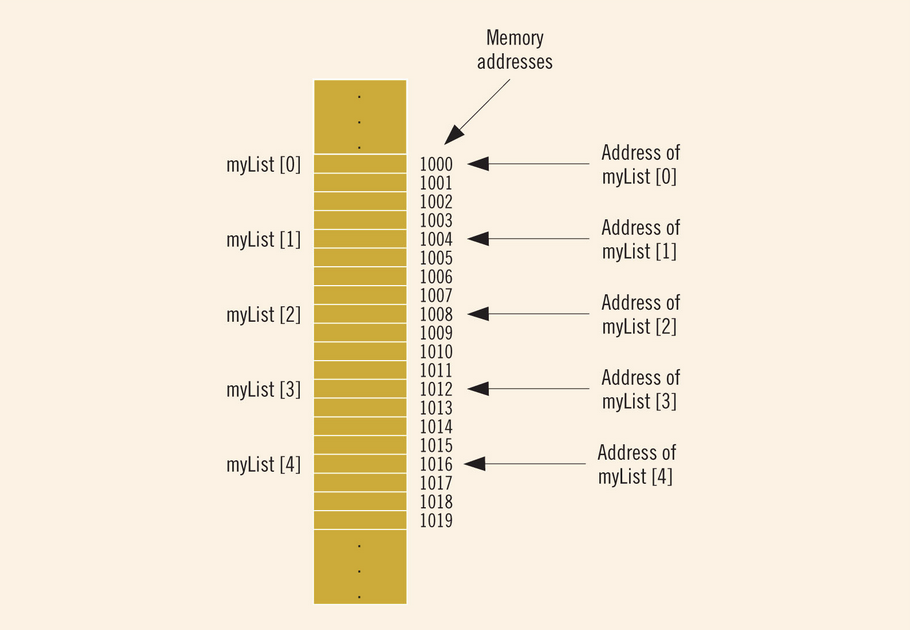
\includegraphics[width=0.9\textwidth]{arr-addy-com-mem.png}
\end{center}

% SECTION 1.9 %
\subsection{Functions Cannot Return a Value of the Type Array}
C++ does not allow functions to return a value of type array.

% SECTION 1.10 %
\subsection{Integral Data Type and Array Indices}
C++ allows any integral type to be used as an array index.

\begin{lstlisting}[caption={Improved Code Readability}]
  enum paintType { GREEN, RED, BLUE, BROWN, WHITE, ORANGE, YELLOW };
  double paintSale[7];

  paintSale[RED] = paintSale[RED] + 75.69;
\end{lstlisting}

% SECTION 1.11 %
\subsection{Other Ways to Declare Arrays}

\begin{lstlisting}[caption={Declaration Using Existing Variable}]
  const int NO_OF_STUDENTS = 20;
  int testScores[NO_OF_STUDENTS];
\end{lstlisting}

\begin{lstlisting}[caption={Declaration with \texttt{using}}]
  const int SIZE = 50;        // Line 1
  using list = double[SIZE];  // Line 2
  list yourList;              // Line 3
  list myList;                // Line 4
\end{lstlisting}

% SECTION 2 %
\section{Searching an Array for a Specific Item}
\textbf{Sequential Search} (\textit{linear search}):
\begin{enumerate}
  \item Searching a list for a given item, starting from the first element.
  \item Compare each element in the array with the value being searched.
  \item Continue to search until item is found or no more data is left. 
\end{enumerate}

\begin{lstlisting}[caption={Simple Array Search}]
  int seqSearch(const int list[], int listLength, int searchItem) {
    int  loc   = 0;
    bool found = false;

    while (loc < listLength && !found) {
      if (list[loc] == searchItem) {
        found = true;
      } else {
        ++loc;
      }
    }

    return found ? loc : -1;
  }
\end{lstlisting}

% SECTION 3 %
\section{Sorting}
\textbf{Selection Sort} is rearranging the list by selecting an element and
moving it to its proper position.

\begin{enumerate}
  \item Find the smallest element in the unsorted portion of the list.
  \item Move it to the top of the unsorted portion by swapping with current
    element.
  \item Start again with the rest of the list.
\end{enumerate}

\begin{center}
    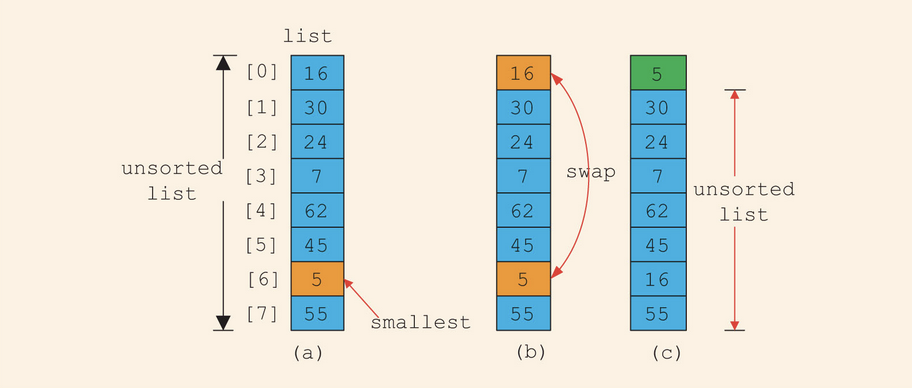
\includegraphics[width=0.9\textwidth]{1D-sel-sort.png}
\end{center}

% SECTION 4 %
\section{Auto Declaration and Range-Based \texttt{for} Loops}
Modern C++ allows for \textbf{Auto} declaration of variables
\begin{itemize}
  \item Data type does not need to be specified.
\end{itemize}

\begin{lstlisting}
  auto num = 15;
\end{lstlisting}

The compiler deduces \texttt{num} to be of type \texttt{int}.

\begin{lstlisting}[caption={Range-Based \texttt{for} Loop}]
  double list[25];
  double sum = 0;

  for (double num : list) {  // read as "for each num in list"
      sum += num;
  }
\end{lstlisting}

% SECTION 5 %
\section{C-Strings (Character Arrays)}
A \textbf{Character Array} is an array whose components are of type
\texttt{char}.

\begin{itemize}
  \item C-strings are \textit{null-terminated} (\texttt{'\\0'}) character arrays.
  \item Examples
    \begin{itemize}
      \item 'A' is the character A
      \item "A" is the C-string A
      \item \textit{Note}: "A" represents two characters. 'A' and \texttt{'\\0'}.
    \end{itemize}
\end{itemize}

\begin{lstlisting}[caption={C-String Declaration}]
  char name[16];
\end{lstlisting}

C-strings are null-terminated and \texttt{name} has 16 components, the largest
string it can store has 15 characters. If you store a string whose length is
less than the array size, the last components are unused.

\begin{lstlisting}[caption={Omitting Size of Array During Initialization}]
  char name[] = "John";
\end{lstlisting}

Declares an array of length \textit{5} and stores the C-string "John" in the
array. Useful \texttt{string} functions:

\begin{itemize}
  \item \texttt{strcopy}
  \item \texttt{strncpy}
  \item \texttt{strcmp}
  \item \texttt{strlen}
\end{itemize}

% SECTION 5.1 %
\subsection{\texttt{string} Comparison}
C-Strings are compared character by character using the collating system
sequence. Use the \texttt{strcmp} function to compare strings.

\vspace{8pt}

If using ASCII char set:
\begin{itemize}
  \item "Air" \textless{} "Boat"
  \item "Air" \textless{} "An"
  \item "Bill" \textless{} "Billy"
  \item "Hello" \textless{} "hello"
\end{itemize}

% SECTION 5.2 %
\subsection{Reading and Writing Strings}
Most array rules apply to C-strings (which are \texttt{char} arrays). However,
C++ \textbf{DOES} allow aggregate ops for the input and output of C-strings.


% SECTION 5.3 %
n\subsection{\texttt{string} Input}
\begin{lstlisting}[caption={String Input Example}]
  cin >> name;
\end{lstlisting}

Stores the next input C-string into \texttt{name}.

\begin{lstlisting}[caption={Read Strings with Blanks with \texttt{get}}]
  cin.get(str, m + 1);
\end{lstlisting}

\begin{itemize}
  \item When executed, stores the next \texttt{m} characters into \texttt{str}, but the
newline character is not stored.
  \item If input string has fewer than \texttt{m} characters, reading stops at
    newline character.
\end{itemize}

% SECTION 5.4 %
\subsection{\texttt{string} Output}
\begin{lstlisting}[caption={String Output Example}]
  cout << name;
\end{lstlisting}

\begin{itemize}
  \item \texttt{<<} continues to write the contents of \texttt{name} until it
    finds a \texttt{null} character.
  \item If \texttt{name} does not contain a \texttt{null} character, then
    strange output may occur as it will continue to output data from memory until a
    \texttt{null} character is found.
\end{itemize}


% SECTION 5.5 %
\subsection{\texttt{string} Type and Input/Output Files}
Argument to open function must be a null-terminated string (a C-string).

\begin{itemize}
  \item If using a string var for the name of an I/O file, the value must first
    be converted to a C-string before calling \texttt{open}.
  \item Use the \texttt{c\_str} function to convert.
\end{itemize}

\begin{lstlisting}[caption={\texttt{c\_str} Syntax}]
  strVar.c\_str();
\end{lstlisting}

Where \texttt{strVar} is a variable of type \texttt{string}.


% SECTION 6 %
\section{Parallel Arrays}
Two (or more) arrays are called \textbf{Parallel} if their corresponding
comonents hold related information.


\begin{lstlisting}[caption={Parallel Array Example}]
  // Stores the values from a 2 column data set file into 2 separate arrays.
  // Each index of each array refers to the same student (therefore parallel).
  int noOfStudents = 0;

  infile >> studentId[noOfStudents] >> courseGrade[noOfStudents];

  while (inFile && noOfStudents < 50) {
    noOfStudents++;
    inFile >> studentId[noOfStudents]
    >> courseGrade[noOfStudents];
  }
\end{lstlisting}

% SECTION 7 %
\section{Two- and Multidimensional Arrays}

\begin{center}
    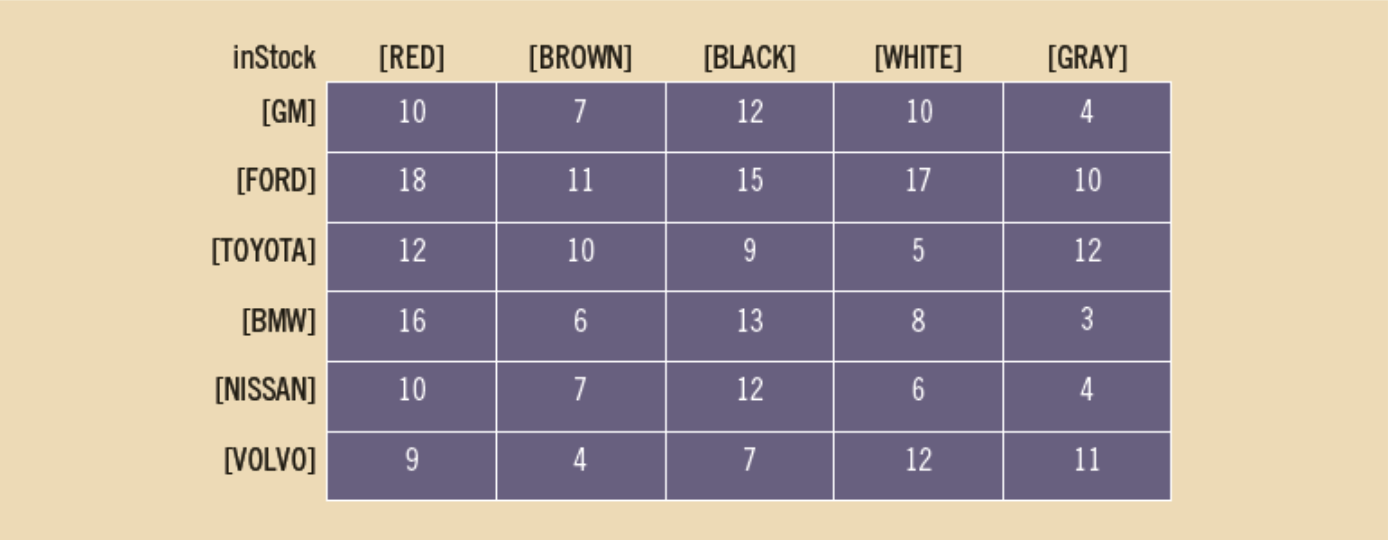
\includegraphics[width=0.9\textwidth]{nD-arr-data-ex.png}
\end{center}

Storing the data set above would require a 1D array of 30 components of type
\texttt{int}. The first five of which would store the first row of the table,
then the next 5, and so on.
\begin{itemize}
  \item This allows you to simulate the table within a 1D array.
  \item Not efficient and can be messy and hard to manage.
\end{itemize}

\textbf{Two-dimensional Arrays} are a collection of a fixed number of components
arranged in rows and columns, where all components are of the same type.

\begin{lstlisting}[caption={Two-Dimensional Array Syntax}]
  dataType arrayName[intExp1] [intExp2];
\end{lstlisting}

Where, \texttt{intExp1} and \texttt{intExp2} are constant expressions yielding
positive integer values.

\begin{lstlisting}[caption={Two-Dimensional Array Example}]
  double sales[10] [5];
\end{lstlisting}

\begin{itemize}
  \item The \textit{rows} are numbered 0-9
  \item The \textit{columns} are numbered 0-4
\end{itemize}

\begin{center}
    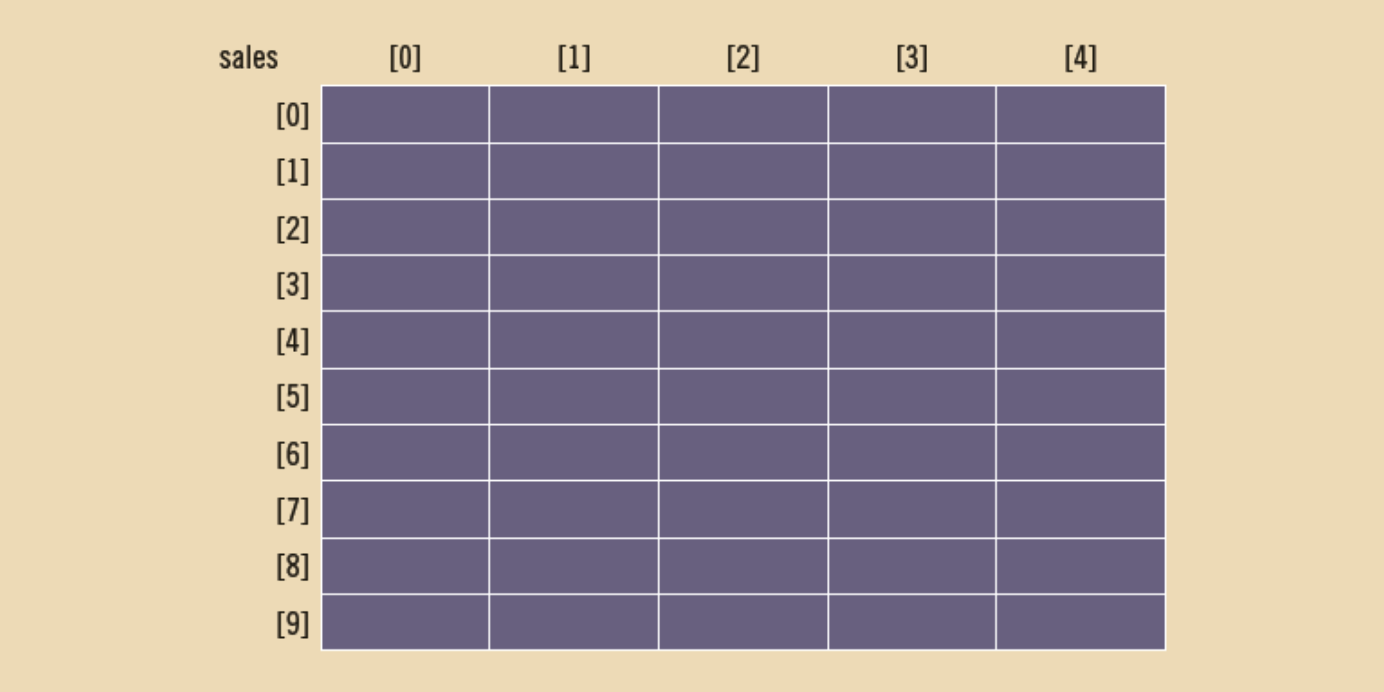
\includegraphics[width=0.9\textwidth]{nD-arr-declaration-table.png}
\end{center}

% SECTION 7.1 %
\subsection{Accessing Array Components}

\begin{lstlisting}[caption={Two-Dimensional Array Indexing Syntax}]
  arrayName[indexExp1] [indexExp2];
\end{lstlisting}

Where, \texttt{intExp1} and \texttt{intExp2} are constant expressions yielding
positive integer values.

\begin{itemize}
  \item \texttt{intExp1} specifies the row position.
  \item \texttt{intExp2} specifies the column position.
\end{itemize}

\begin{lstlisting}[caption={Two-Dimensional Array Indexing Example}]
  sales[5][3] = 25.75;
\end{lstlisting}

Stores \texttt{25.75} into row number 5 and column number 3 of the array
/texttt{sales}.

\begin{center}
    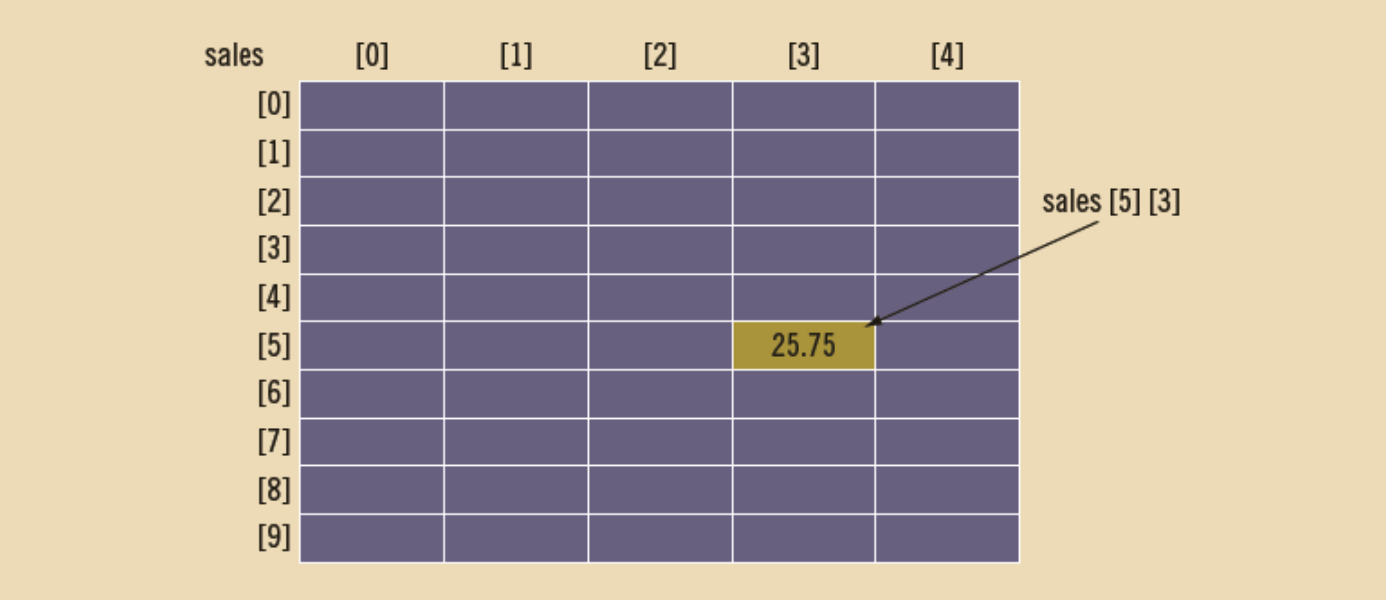
\includegraphics[width=0.9\textwidth]{nD-arr-sales-ex.png}
\end{center}

\begin{lstlisting}[caption={Two-Dimensional Array Indexing With Vars Example}]
  sales[i][j] = 25.75;
\end{lstlisting}

% SECTION 7.2 %
\subsection{Two-Dimensional Array Initialization During Declaration}
\begin{lstlisting}[caption={Two-Dimensional Array Initialization Example}]
  int board[4][3] = {
    {2, 3, 1},
    {15, 25, 13},
    {20, 4, 7},
    {11, 18, 14}
  };
\end{lstlisting}

\begin{center}
    
\includegraphics[width=0.9\textwidth]{2D-arr-board-init.png}
\end{center}

To initialize a two-dimensional array when it is declared:
\begin{enumerate}
  \item The elements of each row are all enclosed within one set of curly
    braces, separated by commas.
  \item Set of all rows is enclosed in curly braces.
  \item For num arrays, if all components od a row are not specified, the
    unspecified components are initialized to \texttt{0}. At least one value is
    needed to initialize all the components of a row.
\end{enumerate}

% SECTION 7.3 %
\subsection{Two-Dimensional Arrays and Enumeration Types}
You can also use enumeration type for array indices.

\begin{lstlisting}[caption={Enumeration Type in Two-Dimensional Arrays Example}]
  const int NUMBER_OF_ROWS = 6;
  const int NUMBER_OF_COLUMNS = 5;

  enum carType {GM, FORD, TOYOTA, BMW, NISSAN, VOLVO};
  enum colorType {RED, BROWN, BLACK, WHITE, GRAY};

  int inStock[NUMBER_OF_ROWS][NUMBER_OF_COLUMNS];

  // Inserting a value into the 2D array
  inStock[1][3] = 15;

  // This is equivalent to the above
  inStock[FORD][WHITE] = 15;
\end{lstlisting}

\begin{center}
    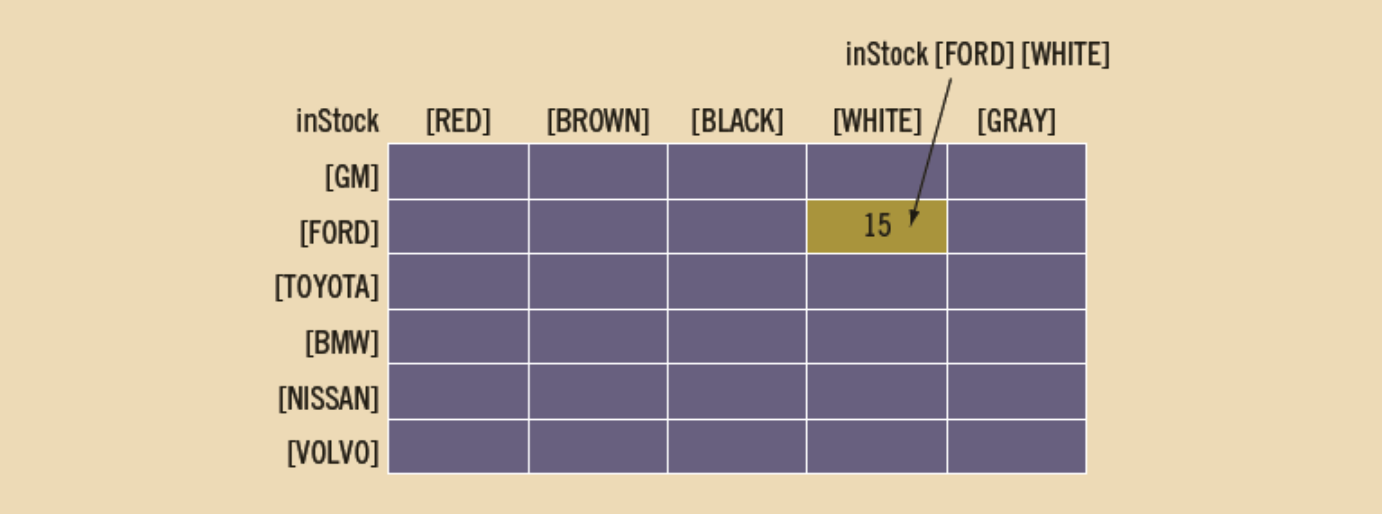
\includegraphics[width=0.9\textwidth]{2D-arr-inStock-ex.png}
\end{center}

% SECTION 7.4 %
\subsection{Processing Two-Dimensional Arrays}
A two-dimensional array can be processed in four ways:
\begin{enumerate}
  \item Process a single element.
  \item Process the entire array.
  \item Process a particular row of the array, called \textbf{Row 
    Processing}
  \item Process a particular column of the array, called \textbf{Column
    Processing}
\end{enumerate}

Each row and column of a two-dimensional array is a one-dimensional array.
\begin{itemize}
  \item To process, use algorithms similar to processing one-dimensional arrays.
\end{itemize}

% SECTION 7.5 %
\subsection{Initialization}
\begin{lstlisting}[caption={Initialize Row Number 4}]
  row = 4;

  for (col = 0; col < NUMBER_OF_COLUMNS; ++col) {
    matrix[row][col] = 0;
  }
\end{lstlisting}

\begin{lstlisting}[caption={Initialize Entire Matrix}]
  for (row = 0; row < NUMBER_OF_ROWS; ++row)  {
    for (col = 0; col < NUMBER_OF_COLUMNS; ++col) {
      matrix[row][col] = 0;
    }
  }
\end{lstlisting}

% SECTION 7.6 %
\subsection{Print}
\begin{lstlisting}[caption={Output Components of a Two-Dimensional Array}]
  for (row = 0; row < NUMBER_OF_ROWS; ++row) { 
    for (col = 0; col < NUMBER_OF_COLUMNS; ++col) {
      cout << setw(5) << matrix[row][col] << ' '; 
      cout << '\n';
    }
  }
\end{lstlisting}

% SECTION 7.7 %
\subsection{Input}
\begin{lstlisting}[caption={Adding Input to 4th Row}]
  row = 4;

  for (col = 0; col < NUMBER_OF_COLUMNS; ++col) {
    cin >> matrix[row][col];
  }
\end{lstlisting}

\begin{lstlisting}[caption={Adding Input to Each Component of Matrix}]
  for (row = 0; row < NUMBER_OF_ROWS; ++row) {
    for (col = 0; col < NUMBER_OF_COLUMNS; ++col) {
      cin >> matrix[row][col];
    }
  }
\end{lstlisting}

% SECTION 7.8 %
\subsection{Sum by Row}
\begin{lstlisting}[caption={Find the Sum of Row Number 4}]
  sum = 0;
  row = 4;

  for (col = 0; col < NUMBER_OF_COLUMNS; ++col) {
    sum += matrix[row][col];
  }
\end{lstlisting}

% SECTION 7.9 %
\subsection{Sum by Column}
\begin{lstlisting}[caption={Find Sum of Individual Columns}]
  // Sum of each individual row 
  for (row = 0; row < NUMBER_OF_ROWS; ++row) {
    sum = 0;

    for (col = 0; col < NUMBER_OF_COLUMNS; ++col) {
      sum += matrix[row][col];
    }

    cout << "Sum of row " << (row + 1) << " = " << sum << '\n';
  }
\end{lstlisting}

% SECTION 7.10 %
\subsection{Largest Element in Each Row and Each Column}
\begin{lstlisting}[caption={Algorithm To Find Largest Element in Each Row}]
  // Largest element in each row 
  for (row = 0; row < NUMBER_OF_ROWS; ++row) {
    largest = matrix[row][0]; // Assume the first element is largest

    for (col = 1; col < NUMBER_OF_COLUMNS; ++col) {
      if (matrix[row][col] > largest) {
        largest = matrix[row][col];
      }

    cout << "The largest element in row " << row << " = " << largest << '\n';
  }
\end{lstlisting}

% SECTION 7.11 %
\subsection{Passing Two-Dimensional Arrays as Parameters to Functions}
Two-dimensional arrays are passed by reference as parameters to a function.
\begin{itemize}
  \item The base address is passed to the formal parameter.
  \item Stored in \textbf{Row Order Form}.
\end{itemize}

When declaring the array as a formal parameter, omit the size of the first
dimension, but not the second.

% SECTION 7.12 %
\subsection{Array of Strings}
Strings in C++ can be manipulated using either the data type \texttt{string} or
character arrays (C-strings).

% SECTION 7.13 %
\subsection{Array of Strings and the \texttt{string} Type}
\begin{lstlisting}[caption={Array of Strings of 100 Elements}]
  string list[100];
\end{lstlisting}

% SECTION 7.14 %
\subsection{Array of Strings and \texttt{C-Strings}}
\begin{lstlisting}[caption={C-String Array}]
  char list[100][16];

  strcpy(list[1], "Snow White");
\end{lstlisting}

\begin{center}
    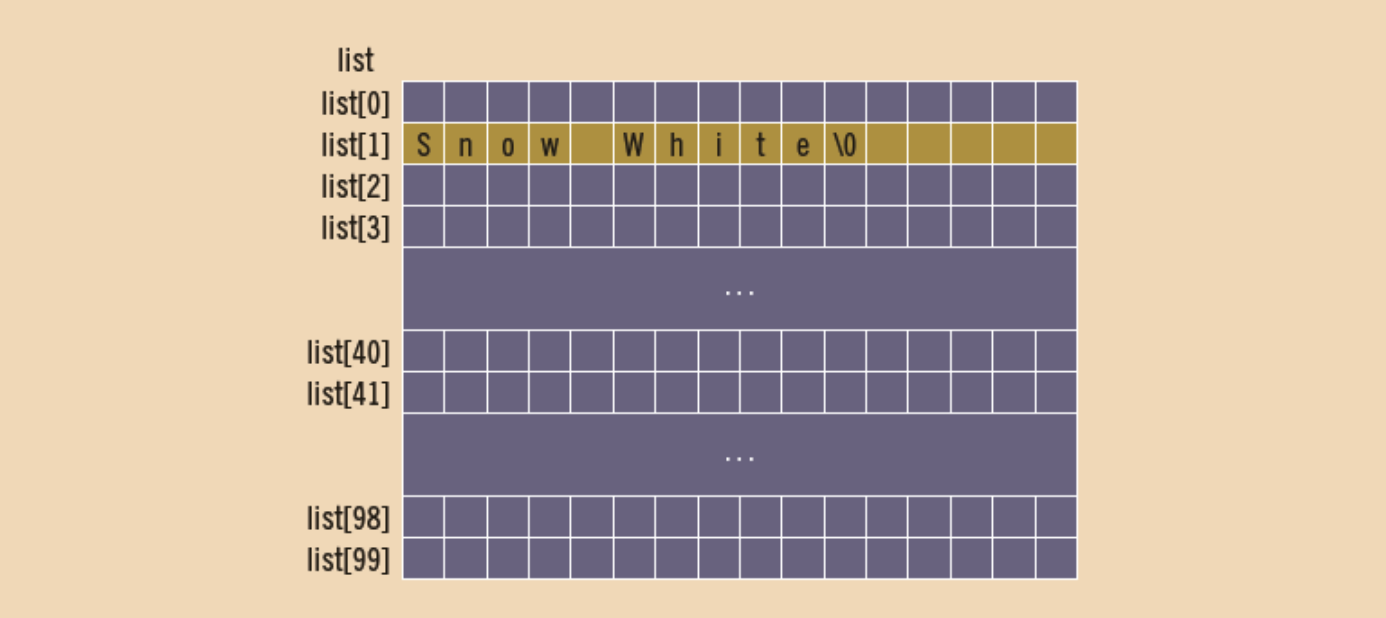
\includegraphics[width=0.9\textwidth]{2D-arr-c-str-matrix.png}
\end{center}

% SECTION 7.15 %
\subsection{Another Way to Declare a Two-Dimensional Array}
Can use \texttt{using} (or \texttt{typedef}) to define a two-dimensional array
data type:

\begin{lstlisting}[caption={\texttt{using} Two-Dimensional Array}]
  const int NUMBER_OF_ROWS = 20;
  const int NUMBER_OF_COLUMNS = 10;

  using tableType = int[NUMBER_OF_ROWS][NUMBER_OF_COLUMNS];

  // Declares array of 20 rows and 10 columns
  tableType matrix;
\end{lstlisting}

% SECTION 7.16 %
\subsection{Multi-Dimensional Arrays}
\textbf{N-Dimensional Array} is a collection of a fixed number of elements
arranged in \textit{n} dimensions, $n >= 1$.

\begin{lstlisting}[caption={Multi-Dimensional Array Syntax}]
  dataType arrayName[intExp1][intExp2]...[intExpN];
\end{lstlisting}

\begin{lstlisting}[caption={Accessing a Multi-Dimensional Array Component}]
  arrayName[indexExp1][indexExp2]...[indexExpN]
\end{lstlisting}

\end{document}
